\usepackage{tikz}
\usepackage{xstring}

% Aquí van todas las figuras en TikZ, hay que asignarlas un numero para poder cambiar todas a la vez.

\newcommand{\figura}[1]{
	\IfEqCase{#1}{
	% PARTE I %
		{hipervisor1}{\figurahipA}
		{hipervisor2}{\figurahipB}
		{hipervisor2real}{\figurahipBfin}
		{hardware}{\figuraHard}
		{sohost1}{\figuraSO}
		{sohost2}{\figuraSOsimpl}
		{hipervisor}{\hipervisor}
		{maqinavirtual}{\maquinavir{0.7}{1}}
		{virtualizacionnat}{\maquinavir{0.3}{0.4} \maquinavir{0.3}{0.4} \maquinavir{0.3}{0.4} \virtualizacionNat}
		{virtualizacionhost}{\virtualizacionHost}
		{vmware}{\fbox{\parbox{70mm}{\textcolor{red}{ESTA FIGURA HAY QUE HACERLA\\ ES COMO LA ÚLTIMA PERO LAS VM ESTAN EL EL SERVIDOR}}}}
	% PARTE II %
		{pizarra}{\pizarra}
		{defarquitectura}{\arqdef}
	}[\PackageError{figura}{Figura no declarada: #1}{}]
}


% Aqui se añaden las figuras %
\newcommand{\figurahipA}{
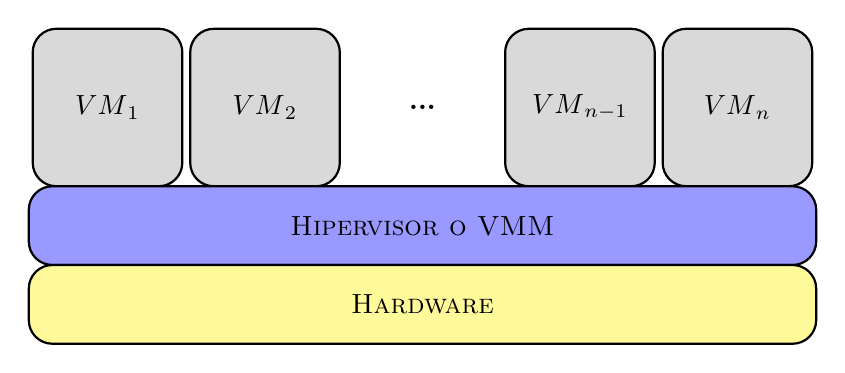
\begin{tikzpicture}
	\draw[rounded corners=3mm, fill=gray!30, thick] (0.05,2) rectangle (1.95,4);
	\draw[rounded corners=3mm, fill=gray!30, thick] (2.05,2) rectangle (3.95,4);
	\draw[rounded corners=3mm, fill=gray!30, thick] (6.05,2) rectangle (7.95,4);
	\draw[rounded corners=3mm, fill=gray!30, thick] (8.05,2) rectangle (9.95,4);
	\draw[rounded corners=3mm, fill={blue!40}, thick] (0,1) rectangle (10,2); 
	\draw[rounded corners=3mm, fill=yellow!40, thick] (0,0) rectangle (10,1); 

	\node at (1,3) {${VM}_1$};
	\node at (3,3) {${VM}_2$};
	\node at (5,3) {\textbf{...}};
	\node at (7,3) {${VM}_{n-1}$};
	\node at (9,3) {${VM}_n$};
	\node at (5,1.5) {\textsc{Hipervisor o VMM}};
	\node at (5,0.5) {\textsc{Hardware}};
\end{tikzpicture}
}

\newcommand{\figurahipB}{
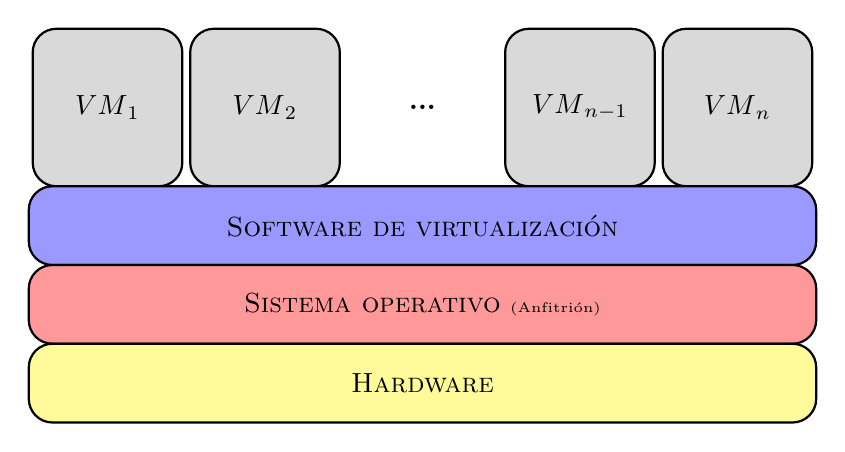
\begin{tikzpicture}
	\draw[rounded corners=3mm, fill=gray!30, thick] (0.05,3) rectangle (1.95,5);
	\draw[rounded corners=3mm, fill=gray!30, thick] (2.05,3) rectangle (3.95,5);
	\draw[rounded corners=3mm, fill=gray!30, thick] (6.05,3) rectangle (7.95,5);
	\draw[rounded corners=3mm, fill=gray!30, thick] (8.05,3) rectangle (9.95,5);
	\draw[rounded corners=3mm, fill={blue!40}, thick] (0,2) rectangle (10,3);
	\draw[rounded corners=3mm, fill={red!40}, thick] (0,1) rectangle (10,2); 
	\draw[rounded corners=3mm, fill=yellow!40, thick] (0,0) rectangle (10,1); 

	\node at (1,4) {${VM}_1$};
	\node at (3,4) {${VM}_2$};
	\node at (5,4) {\textbf{...}};
	\node at (7,4) {${VM}_{n-1}$};
	\node at (9,4) {${VM}_n$};
	\node at (5,2.5) {\textsc{Software de virtualización}};
	\node at (5,1.5) {\textsc{Sistema operativo} {\tiny (Anfitrión)}};
	\node at (5,0.5) {\textsc{Hardware}};
\end{tikzpicture}
}

\newcommand{\figurahipBfin}{
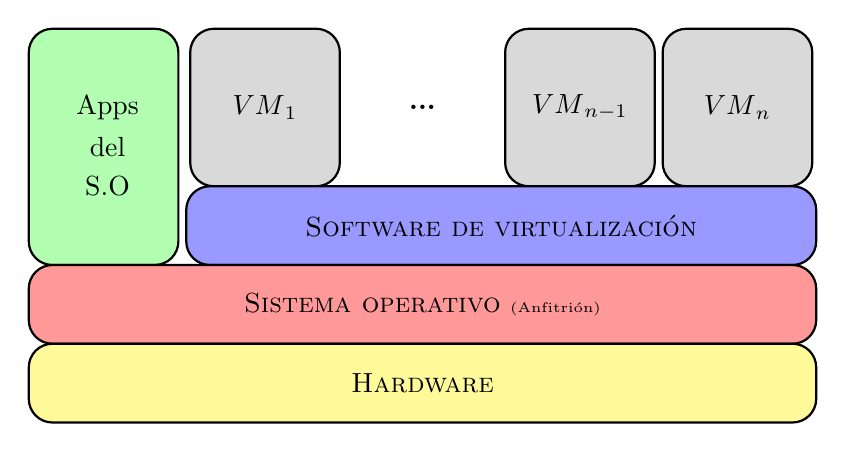
\begin{tikzpicture}
	\draw[rounded corners=3mm, fill=green!30, thick] (0,2) rectangle (1.90,5);
	\draw[rounded corners=3mm, fill=gray!30, thick] (2.05,3) rectangle (3.95,5);
	\draw[rounded corners=3mm, fill=gray!30, thick] (6.05,3) rectangle (7.95,5);
	\draw[rounded corners=3mm, fill=gray!30, thick] (8.05,3) rectangle (9.95,5);
	\draw[rounded corners=3mm, fill={blue!40}, thick] (2,2) rectangle (10,3);
	\draw[rounded corners=3mm, fill={red!40}, thick] (0,1) rectangle (10,2); 
	\draw[rounded corners=3mm, fill=yellow!40, thick] (0,0) rectangle (10,1); 

	\node at (1,4) {Apps};
	\node at (1,3.5) {del};
	\node at (1,3) {S.O};
	\node at (3,4) {${VM}_1$};
	\node at (5,4) {\textbf{...}};
	\node at (7,4) {${VM}_{n-1}$};
	\node at (9,4) {${VM}_n$};
	\node at (6,2.5) {\textsc{Software de virtualización}};
	\node at (5,1.5) {\textsc{Sistema operativo} {\tiny (Anfitrión)}};
	\node at (5,0.5) {\textsc{Hardware}};
\end{tikzpicture}
}

\newcommand{\figuraHard}{
\begin{tikzpicture}
	\draw[rounded corners=3mm, fill=yellow!40, thick] (-0.05,-0.05) rectangle (10.05,3.05);

	\node at (2,2.5) {\textsc{Hardware Real}};
	
	\node at (1.25,1.4) {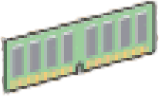
\includegraphics{./images/memoria.png}};
	\node at (1.25,0.5) {\textsc{Memoria}};
	
	\node at (3.75,1.4) {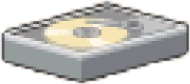
\includegraphics{./images/hdd.png}};
	\node at (3.75,0.5) {\textsc{Disco}};
	
	\node at (6.25,1.4) {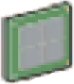
\includegraphics{./images/cpu.png}};
	\node at (6.25,0.5) {\textsc{CPU}};
	
	\node at (8.75,1.4) {
\includegraphics{./images/red.png}};
	\node at (8.75,0.5) {\textsc{Red}};
\end{tikzpicture}
}

\newcommand{\figuraSO}{
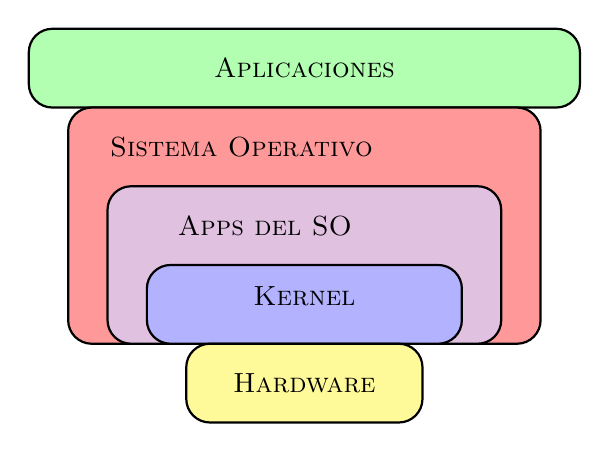
\begin{tikzpicture}
\definecolor{morado}{RGB}{177,100,177}
	\draw[rounded corners=3mm, fill=green!30, thick] (-.50,3) rectangle (6.5,4);
	\draw[rounded corners=3mm, fill=red!40, thick] (0,0) rectangle (6,3);
	\draw[rounded corners=3mm, fill=morado!40, thick] (0.5,0) rectangle (5.5,2);
	\draw[rounded corners=3mm, fill=blue!30, thick] (1,0) rectangle (5,1);
	\draw[rounded corners=3mm, fill=yellow!40, thick] (1.5,-1) rectangle (4.5,0);
	
	\node at (3,3.5) {\textsc{Aplicaciones}};
	\node at (2.2,2.5) {\textsc{Sistema Operativo}};
	\node at (2.5,1.5) {\textsc{Apps del SO}};
	\node at (3,0.6) {\textsc{Kernel}};
	\node at (3,-0.5) {\textsc{Hardware}};
\end{tikzpicture}
}

\newcommand{\figuraSOsimpl}{
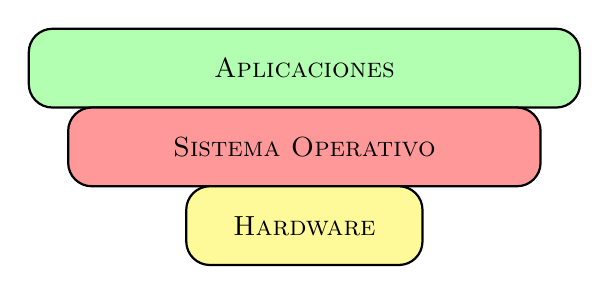
\begin{tikzpicture}
	\draw[rounded corners=3mm, fill=green!30, thick] (-0.5,1) rectangle (6.5,2);
	\draw[rounded corners=3mm, fill=red!40, thick] (0,0) rectangle (6,1);
	\draw[rounded corners=3mm, fill=yellow!40, thick] (1.5,-1) rectangle (4.5,0);
	
	\node at (3,1.5) {\textsc{Aplicaciones}};
	\node at (3,0.5) {\textsc{Sistema Operativo}};
	\node at (3,-0.5) {\textsc{Hardware}};
\end{tikzpicture}
}

\newcommand{\hipervisor}{
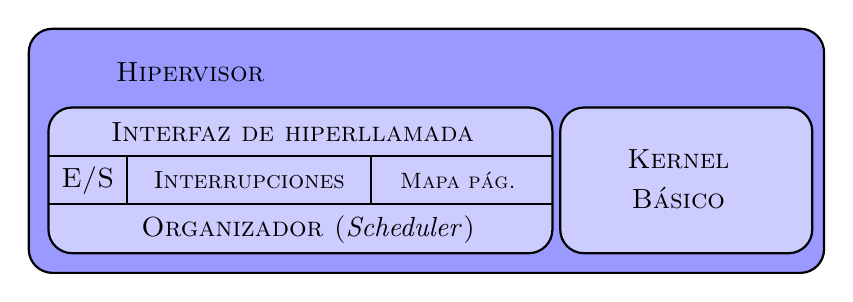
\begin{tikzpicture}
	\draw[rounded corners=3mm, fill=blue!40, thick] (-0.05,-0.05) rectangle (10.05,3.05);
	\draw[rounded corners=3mm, fill=blue!20, thick] (0.2,0.2) rectangle (6.6,2.05);
	\draw[rounded corners=3mm, fill=blue!20, thick] (6.7,0.2) rectangle (9.9,2.05);

	\draw[thick] (0.2,0.82) -- (6.6,0.82);
	\draw[thick] (0.2,1.43) -- (6.6,1.43);
	
	\draw[thick] (1.2,1.43) -- (1.2,0.82);
	\draw[thick] (4.3,1.43) -- (4.3,0.82);
	
	
	\node at (2,2.5) {\textsc{Hipervisor}};
	
	\node at (3.3,1.74) {\textsc{Interfaz de hiperllamada}};
	\node at (0.7,1.125) {\textsc{E/S}};
	\node at (2.75,1.125) {{\small \textsc{Interrupciones}}};
	\node at (5.4,1.125) {{\footnotesize \textsc{Mapa pág.}}};
	\node at (3.5,0.5) {\textsc{Organizador (\emph{Scheduler})}};
	
	\node at (8.2,1.4) {\textsc{Kernel}};
	\node at (8.2,0.9) {\textsc{Básico}};
\end{tikzpicture}
}

\newcommand{\maquinavir}[2]{
\begin{tikzpicture}[scale=#1]
	\draw[rounded corners=3mm, fill=gray!30, thick] (-0.30,-0.3) rectangle (10.3,10);
	\draw[rounded corners=3mm, fill=green!30, thick] (-0.05,6.05) rectangle (10.05,9.05);
	\draw[rounded corners=3mm, fill=red!40, thick] (-0.05,3.05) rectangle (10.05,6.05);		
	\draw[rounded corners=3mm, fill=yellow!40, thick] (-0.05,-0.05) rectangle (10.05,3.05);
	
	\node at (5,9.4) {\scalebox{#2}{{\Large {\textsc{Máquina Virtual}} }}};
	
	\node at (5,7.5) {\scalebox{#2}{{\textsc{Aplicaciones}} }};
	
	\node at (5,4.5) {\scalebox{#2}{{\textsc{Sistema operativo}} }};
	
	\node at (2.7,2.5) {\scalebox{#2}{{{\small \textsc{Hardware Virtual}} }}};
	
	\node at (1.25,1.4) {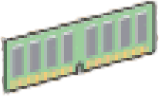
\includegraphics[scale=#1]{./images/memoria.png}};
	\node at (1.25,0.5) {\scalebox{#2}{{\scriptsize \textsc{Memoria}}}};
	
	\node at (3.75,1.4) {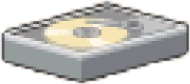
\includegraphics[scale=#1]{./images/hdd.png}};
	\node at (3.75,0.5) {\scalebox{#2}{{\scriptsize \textsc{Disco}}}};
	
	\node at (6.25,1.4) {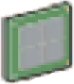
\includegraphics[scale=#1]{./images/cpu.png}};
	\node at (6.25,0.5) {\scalebox{#2}{{\scriptsize \textsc{CPU}}}};
	
	\node at (8.75,1.4) {
\includegraphics[scale=#1]{./images/red.png}};
	\node at (8.75,0.5) {\scalebox{#2}{{\scriptsize \textsc{Red}}}};
\end{tikzpicture}
}


\newcommand{\virtualizacionNat}{
\begin{tikzpicture}
	\draw[rounded corners=3mm, fill={blue!40}, thick] (0,3.05) rectangle (10.5,4); 
	\draw[rounded corners=3mm, fill=yellow!40, thick] (-0.05,-0.05) rectangle (10.5,3.05);
	
	\node at (5,3.5) {\textsc{Hipervisor o VMM}};

	
	\node at (2,2.5) {\textsc{Hardware Real}};
		
	\node at (1.25,1.4) {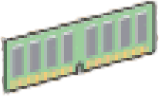
\includegraphics{./images/memoria.png}};
	\node at (1.25,0.5) {\textsc{Memoria}};
		
	\node at (3.75,1.4) {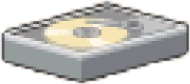
\includegraphics{./images/hdd.png}};
	\node at (3.75,0.5) {\textsc{Disco}};
		
	\node at (6.25,1.4) {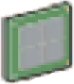
\includegraphics{./images/cpu.png}};
	\node at (6.25,0.5) {\textsc{CPU}};
		
	\node at (8.75,1.4) {
\includegraphics{./images/red.png}};
	\node at (8.75,0.5) {\textsc{Red}};
\end{tikzpicture}
}

\newcommand{\virtualizacionHost}{
\begin{tikzpicture}

	\draw[rounded corners=3mm, fill=gray!30, thick] (11,5) rectangle (14.5,8.2);
	\draw[rounded corners=3mm, fill=yellow!40, thick] (11.05,5.1) rectangle (14.45,5.95);
	\draw[rounded corners=3mm, fill=red!40, thick] (11.05,5.95) rectangle (14.45,6.95);		
	\draw[rounded corners=3mm, fill=green!40, thick] (11.05,6.95) rectangle (14.45,7.95);
	
	\node at (12.75,5.8) { \textsc{\tiny Hardware virtual}};
	\node at (12.75,7.45) {\textsc{\scriptsize Aplicaciones}};
	\node at (12.75,6.45) {\textsc{\tiny Sistema Operativo}};
	\node at (12.75,8.05) {\textsc{\tiny Máquina Virtual}};
	
	\node at (11.5,5.4) {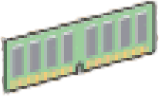
\includegraphics[scale=0.3]{./images/memoria.png}};
	\node at (12.3,5.4) {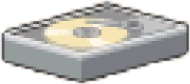
\includegraphics[scale=0.3]{./images/hdd.png}};
	\node at (13.3,5.4) {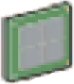
\includegraphics[scale=0.3]{./images/cpu.png}};
	\node at (14.1,5.4) {
\includegraphics[scale=0.3]{./images/red.png}};
	
	\draw[rounded corners=3mm, fill=gray!30, thick] (7,5) rectangle (10.5,8.2);
	\draw[rounded corners=3mm, fill=yellow!40, thick] (7.05,5.1) rectangle (10.45,5.95);
	\draw[rounded corners=3mm, fill=red!40, thick] (7.05,5.95) rectangle (10.45,6.95);		
	\draw[rounded corners=3mm, fill=green!40, thick] (7.05,6.95) rectangle (10.45,7.95);
	
	\node at (8.75,5.8) { \textsc{\tiny Hardware virtual}};
	\node at (8.75,7.45) {\textsc{\scriptsize Aplicaciones}};
	\node at (8.75,6.45) {\textsc{\tiny Sistema Operativo}};
	\node at (8.75,8.05) {\textsc{\tiny Máquina Virtual}};
	
	\node at (7.5,5.4) {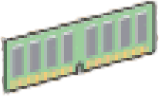
\includegraphics[scale=0.3]{./images/memoria.png}};
	\node at (8.3,5.4) {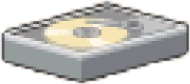
\includegraphics[scale=0.3]{./images/hdd.png}};
	\node at (9.3,5.4) {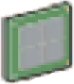
\includegraphics[scale=0.3]{./images/cpu.png}};
	\node at (10.1,5.4) {
\includegraphics[scale=0.3]{./images/red.png}};
		
	\draw[rounded corners=3mm, fill=gray!30, thick] (3,5) rectangle (6.5,8.2);
	\draw[rounded corners=3mm, fill=yellow!40, thick] (3.05,5.1) rectangle (6.45,5.95);
	\draw[rounded corners=3mm, fill=red!40, thick] (3.05,5.95) rectangle (6.45,6.95);		
	\draw[rounded corners=3mm, fill=green!40, thick] (3.05,6.95) rectangle (6.45,7.95);
	
	\node at (4.75,5.8) { \textsc{\tiny Hardware virtual}};
	\node at (4.75,7.45) {\textsc{\scriptsize Aplicaciones}};
	\node at (4.75,6.45) {\textsc{\tiny Sistema Operativo}};
	\node at (4.75,8.05) {\textsc{\tiny Máquina Virtual}};
	
	\node at (3.5,5.4) {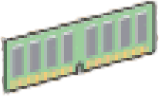
\includegraphics[scale=0.3]{./images/memoria.png}};
	\node at (4.3,5.4) {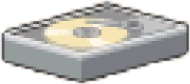
\includegraphics[scale=0.3]{./images/hdd.png}};
	\node at (5.3,5.4) {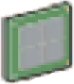
\includegraphics[scale=0.3]{./images/cpu.png}};
	\node at (6.1,5.4) {
\includegraphics[scale=0.3]{./images/red.png}};

	\draw[rounded corners=3mm, fill={blue!40}, thick] (3,4) rectangle (14.5,5);
	\draw[rounded corners=3mm, fill={red!40}, thick] (-0.05,3.05) rectangle (14.5,4);  
	\draw[rounded corners=3mm, fill=yellow!40, thick] (-0.05,-0.05) rectangle (14.5,3.05);
	\draw[rounded corners=3mm, fill=green!30, thick] (-0.05,4) rectangle (2.85,8.2);
	
	\node at (1.45,6.5) {Apps};
	\node at (1.45,6) {del};
	\node at (1.45,5.5) {S.O};
	
	\node at (8.5,4.5) {\textsc{Hipervisor o VMM}};
	\node at (7.25,3.5) {\textsc{Sistema Operativo}};
	\node at (2,2.5) {\textsc{Hardware Real}};
			
		\node at (1,1.4) {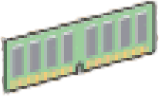
\includegraphics{./images/memoria.png}};
		\node at (1,0.5) {\textsc{Memoria}};
			
		\node at (5.5,1.4) {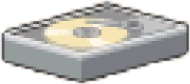
\includegraphics{./images/hdd.png}};
		\node at (5.5,0.5) {\textsc{Disco}};
			
		\node at (9.5,1.4) {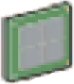
\includegraphics{./images/cpu.png}};
		\node at (9.5,0.5) {\textsc{CPU}};
			
		\node at (13.5,1.4) {
\includegraphics{./images/red.png}};
		\node at (13.5,0.5) {\textsc{Red}};
\end{tikzpicture}
}


\newcommand{\pizarra}{
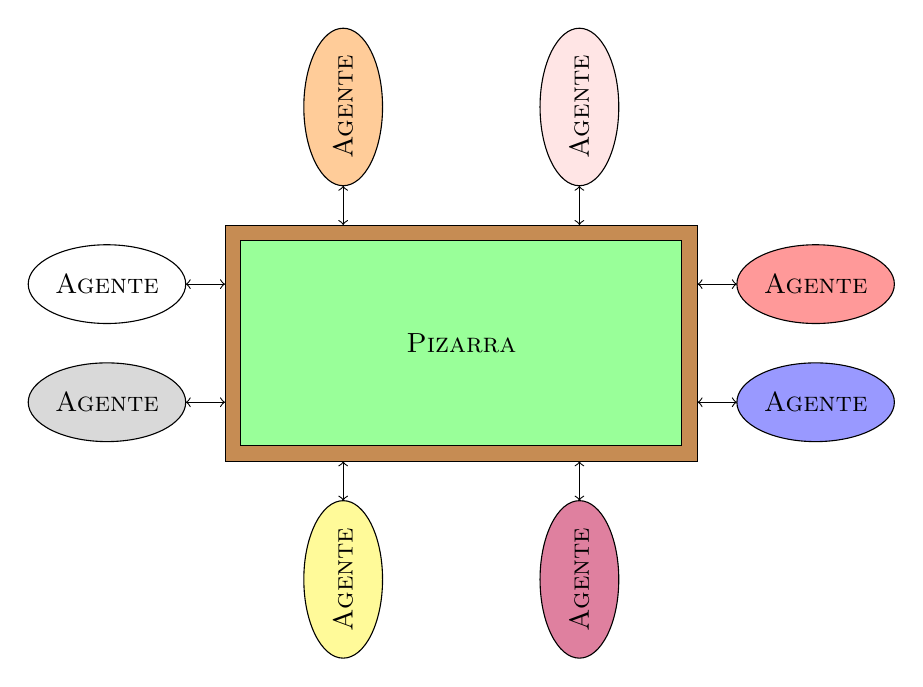
\begin{tikzpicture}
	\draw[fill=brown!90] (0,0) rectangle (6,3);
	\draw[fill=green!40] (0.2, 0.2) rectangle (5.8,2.8);
	
	\draw[fill=red!40] (7.5,2.25) ellipse (1cm and 0.5cm);
	\draw[fill=blue!40] (7.5,0.75) ellipse (1cm and 0.5cm);
	\draw[fill=yellow!40] (1.5,-1.5) ellipse (0.5cm and 1cm);
	\draw[fill=purple!50] (4.5,-1.5) ellipse (0.5cm and 1cm);
	\draw[fill=gray!30] (-1.5,0.75) ellipse (1cm and 0.5cm);
	\draw[fill=white!40] (-1.5,2.25) ellipse (1cm and 0.5cm);
	\draw[fill=orange!40] (1.5,4.5) ellipse (0.5cm and 1cm);
	\draw[fill=pink!40] (4.5,4.5) ellipse (0.5cm and 1cm);
	
	\draw[<->] (6,0.75) -- (6.5,0.75);
	\draw[<->] (6,2.25) -- (6.5,2.25);
	\draw[<->] (1.5,3) -- (1.5,3.5);
	\draw[<->] (4.5,3) -- (4.5,3.5);
	\draw[<->] (0,0.75) -- (-0.5,0.75);
	\draw[<->] (0,2.25) -- (-0.5,2.25);
	\draw[<->] (1.5,-0.5) -- (1.5,0);
	\draw[<->] (4.5,-0.5) -- (4.5,0);
	
	\node at (3,1.5) {\textsc{Pizarra}};
	\node at (7.5,2.25) {\textsc{Agente}};
	\node at (7.5,0.75) {\textsc{Agente}};
	\node[rotate=90] at (1.5,-1.5) {\textsc{Agente}};
	\node[rotate=90] at (4.5,-1.5) {\textsc{Agente}};
	\node at (-1.5,0.75) {\textsc{Agente}};
	\node at (-1.5,2.25) {\textsc{Agente}};
	\node[rotate=90] at (1.5,4.5) {\textsc{Agente}};
	\node[rotate=90] at (4.5,4.5) {\textsc{Agente}};
\end{tikzpicture}
}

\newcommand{\arqdef}{
\begin{tikzpicture}[scale=0.8]
	\node at (0,0) {
\includegraphics[scale=0.3]{./images/computer.png}};
	\node at (0,-1) {Agente 1};
	
	\node at (0,-2) {
\includegraphics[scale=0.3]{./images/computer.png}};
	\node at (0,-3) {Agente 2};
	
	\node at (0,-4) {$\mathbf{\vdots}$};
	
	\node at (0,-5) {
\includegraphics[scale=0.3]{./images/computer.png}};
	\node at (0,-6) {Agente n};
	
	\node at (4,-3) {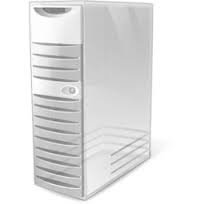
\includegraphics[scale=0.3]{./images/servidor.jpg}};
	\node at (4,-5) {Pizarra};
	
	\node at (8,-3) {
\includegraphics[scale=0.05]{./images/db.png}};
	\node at (8,-4.5) {Base de datos};
	
	\draw (1,0) -- (3,-3);
	\draw (1,-2) -- (3,-3);
	\draw (1,-5) -- (3,-3);
	
	\draw (5,-3) -- (7,-3);


\end{tikzpicture}
}
